We have implemented a suite of tools for analysis of error for all of the aforementioned Langevin Monte Carlo algorithms. This section contains a selection of results, as well as a description of error metrics available and any other design choices made. The \textsc{Python} code and a how-to-use guide can be found at the following
\textsc{url}: \\

   \centerline{ \url{https://github.com/Tom271/LangevinMC}}


\subsection{Results}

\begin{figure}[H]
\centering
  \begin{minipage}[b]{0.49\textwidth}
  \centering
    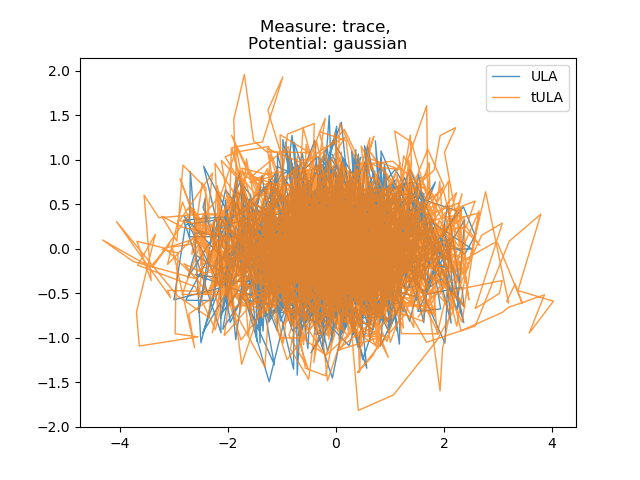
\includegraphics[width=\textwidth]{Figures/ula_tula_step_01.png}
  \end{minipage} %
  \begin{minipage}[b]{0.49\textwidth}
  \centering
    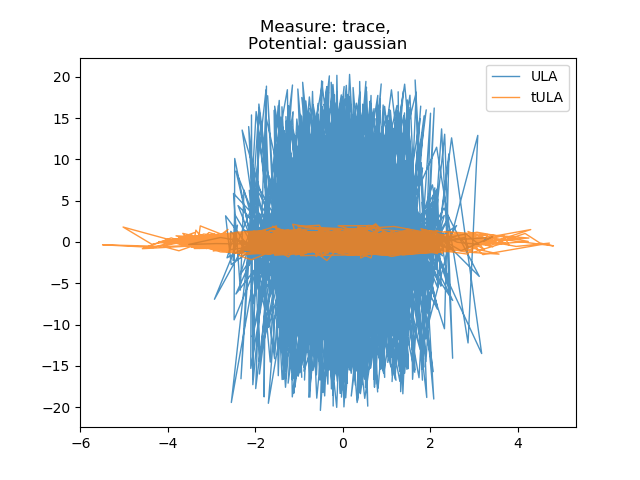
\includegraphics[width=\textwidth]{Figures/ula_tula_step_02.png}
  \end{minipage}
   \caption{\textbf{Demonstration of the stiffness problem with \texttt{ULA}}, resolved by taming. Both \texttt{ULA} and \texttt{tULA} work well for step size $h = 0.1$ on the left, however \texttt{ULA} becomes stiff for a larger step size $h = 0.2$ on the right. For ever higher step sizes, \texttt{ULA} diverges. The distribution here is Gaussian with covariance matrix $\text{diag}(1.0, 0.1)$.}
\end{figure}

\begin{figure}[H]
\centering
  \begin{minipage}[b]{0.49\textwidth}
  \centering
    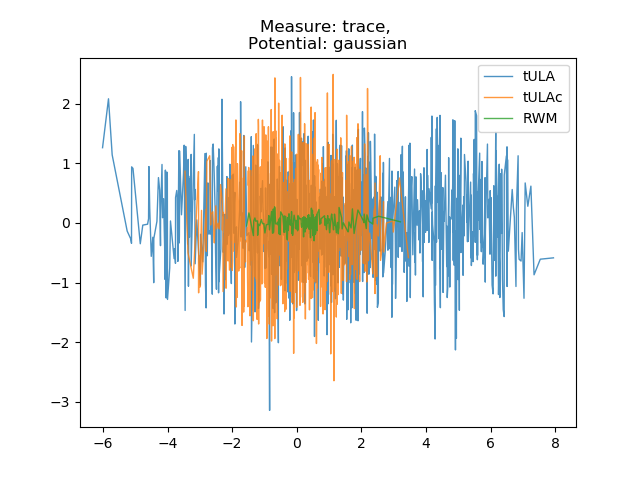
\includegraphics[width=\textwidth]{Figures/tula_tulac_rwm_stiff.png}
  \end{minipage} %
   \caption{\textbf{Coordinate-wise taming} can deal with stiffness in one axis (Ill-conditioned Gaussian distribution with covariance $\text{diag}(1.0, 0.01)$).}
\end{figure}



\begin{figure}[H]
\centering
  \begin{minipage}[b]{0.49\textwidth}
  \centering
    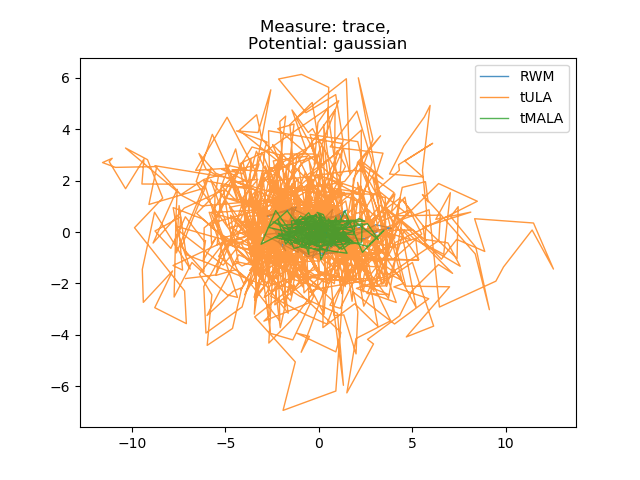
\includegraphics[width=\textwidth]{Figures/tula_tmala_step_1.png}
  \end{minipage} %
  \begin{minipage}[b]{0.49\textwidth}
  \centering
    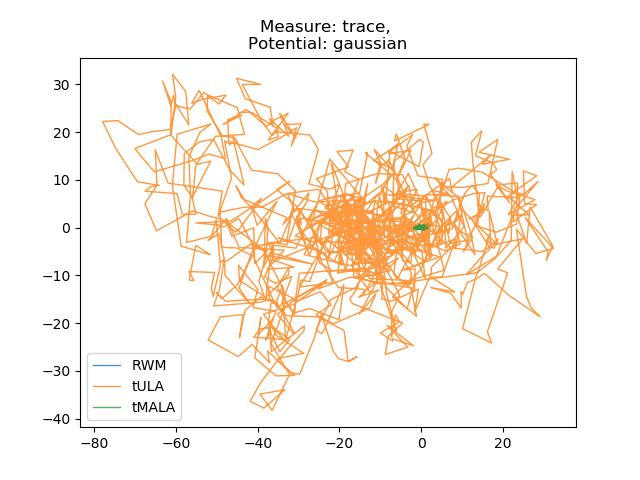
\includegraphics[width=\textwidth]{Figures/tula_tmala_step_10.png}
  \end{minipage}
   \caption{\textbf{Trade-off between rejection-based algorithms and \texttt{tULA} for large step-sizes} ($h = 1$ on the left and $h = 10$ on the right, distribution is Gaussian with covariance matrix $\text{diag}(1.0, 0.1)$). With increasing step size, even \texttt{tULA} starts to suffer from stiffness problems. Rejection-based algorithms resolve the issue, however, their acceptance rate drops very low ($\approx 0.2$ on the left and $\approx 0.03$ on the right). }
\end{figure}



\begin{figure}[H]
\centering
  \begin{minipage}[b]{0.32\textwidth}
  \centering
    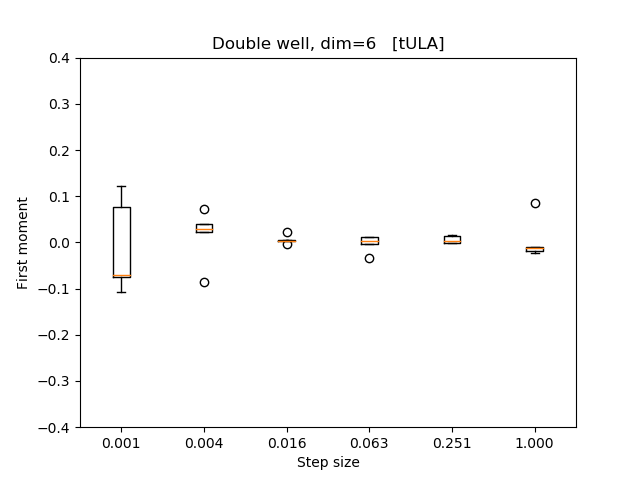
\includegraphics[width=\textwidth]{Figures/tula_fm.png}
  \end{minipage} %
  \begin{minipage}[b]{0.32\textwidth}
  \centering
    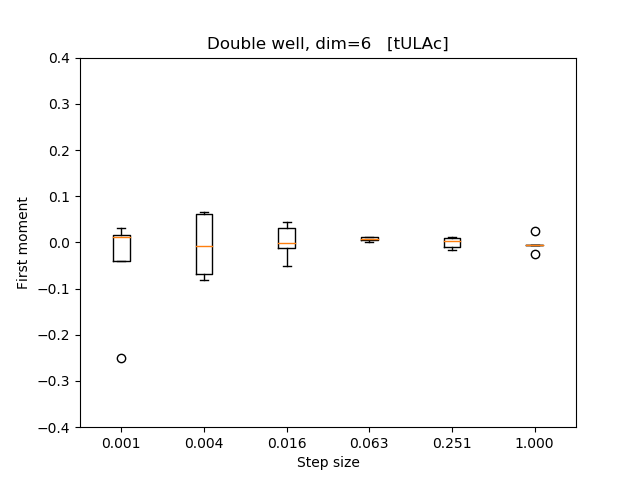
\includegraphics[width=\textwidth]{Figures/tulac_fm.png}
  \end{minipage} %
  \begin{minipage}[b]{0.32\textwidth}
  \centering
    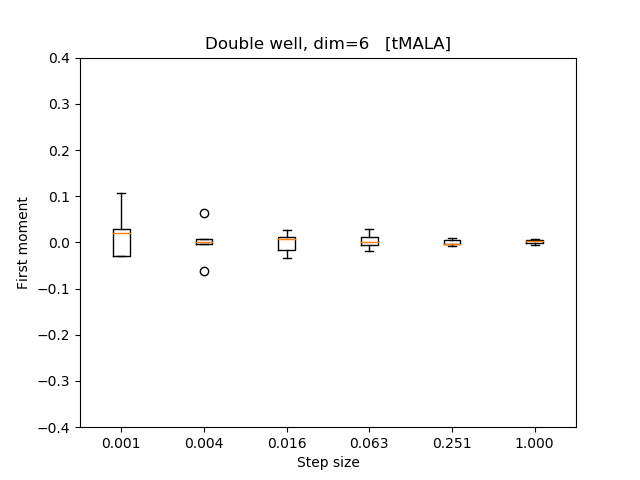
\includegraphics[width=\textwidth]{Figures/tmala_fm.png}
  \end{minipage}
   \caption{Comparison of \texttt{tULA}, \texttt{tULAc} and \texttt{tMALA} for the first moment evolving as a function of step size.}
\end{figure}


\begin{figure}[H]
\centering
  \begin{minipage}[b]{0.32\textwidth}
  \centering
    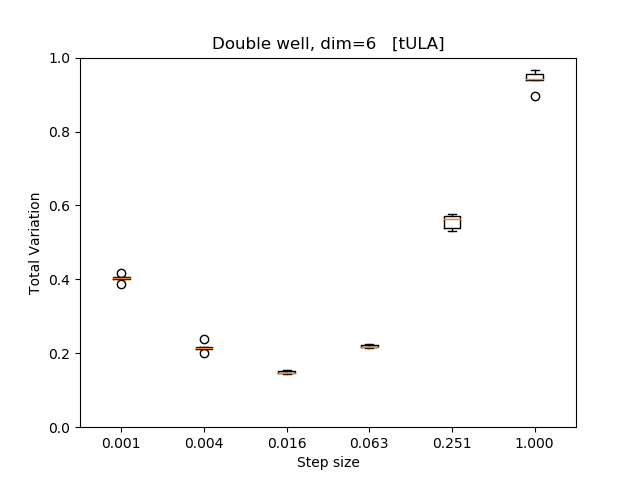
\includegraphics[width=\textwidth]{Figures/tula_tv.png}
  \end{minipage} %
  \begin{minipage}[b]{0.32\textwidth}
  \centering
    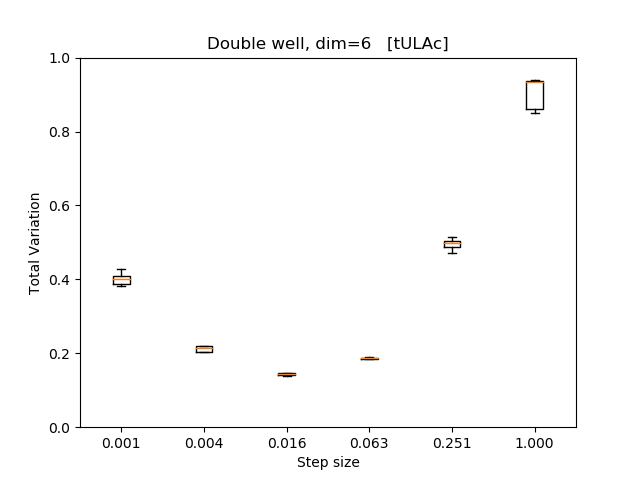
\includegraphics[width=\textwidth]{Figures/tulac_tv.png}
  \end{minipage} %
  \begin{minipage}[b]{0.32\textwidth}
  \centering
    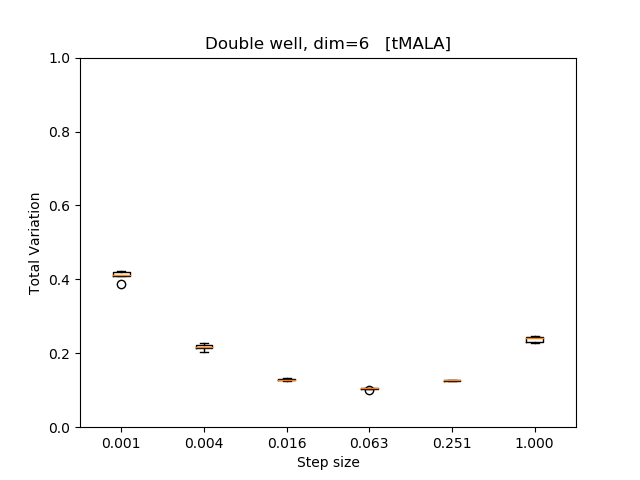
\includegraphics[width=\textwidth]{Figures/tmala_tv.png}
  \end{minipage}
   \caption{Comparison of \texttt{tULA}, \texttt{tULAc} and \texttt{tMALA} for the total variation error evolving as a function of step size.}
\end{figure}




\subsection{Sampling approaches}

Throughout this project, we have encountered two main approaches for sampling. To obtain a set of samples, one may:

\begin{itemize}
    \item Run a single chain, discard a certain amount of the initial values (the burn-in period) and keep the rest, with possible thinning\footnote{To thin the chain, one only retains every $k$-th sample for some $k$.} to reduce autocorrelation. This is used for practical sampling.
    \item Run multiple chains and retain their final $N$-th value only. This is useful for verification/establishment of non-asymptotic bounds.
\end{itemize}

To accommodate for both possibilities, given positive integers $b, N_{\text{chains}}, N$ and a set $I \subset \mathbb \{1, 2, \dots, N - b\}$ of indices, our program aggregates samples with indices in $\{i+b\ |\ i \in I\} $  from $ N_{\text{chains}}$ independent chains.

\subsection{Estimating error}

In the following, let $\pi$ be the pdf of true distribution from which we attempt to sample and $X = \{x_i\}_{i=1}^N$ denote the collection of samples collected by a sampling algorithm. The notation $x_i(d)$ will be used to refer to the $d$-th coordinate of $x_i$. We also denote by $\{m_d\}_{d=1}^D$ and $\{M_d\}_{d=1}^D$ the coordinate-wise minimums and maximums among $x_i$, that is:

$$ 
    m_d = \min \{x_i(d)\}_{i=1}^N \ \ \text{ and } \ \ M_d = \max \{x_i(d)\}_{i=1}^N
$$

For some of the error estimation methods, it will be necessary to construct multi-dimensional histograms. For this purpose, we define the following set of points (this is a minimal mesh that spans all of the samples):

\begin{align*}
    \#_X := \Big\{ \left(c_1^{(k_1)}, c_2^{(k_2)}, \dots, c_D^{(k_D)}\right)\ |\ &(k_1, k_2, \dots, k_D) \in \lbrace 0, 1, \dots, \text{bins - 1}\rbrace^D, \ c_d^{(k_d)} \\
    &= m_d + \left(k_d + \frac 1 2\right) \frac{M_d - m_d}{\text{bins}} \Big\}
\end{align*}

where $bins$ is a parameter describing the fineness of the mesh. The histogram of the collection of samples $X$ will be understood to be the following function $h: \#_X \rightarrow \mathbb R$:

$$
    h(c) = |\{x \in X\ |\ \arg \min_{c' \in \#_X} \norm{c' - x} = c \}|
$$

i.e. count of points $x$ such that the closes point of mesh to $x$ is $c$. This defines the discrete probability measure 

$$H_X := \sum_{c \in \#_X} \frac {h(c)} N   \delta_c,$$

which we will understand to be the sampled approximation of the true distribution from which we are sampling. Finally, denote also by $Z$ the sum of the true distribution pdf values over the values of the mesh.

\[Z := \sum_{c \in \#_X} \pi(c)\]



\subsubsection{The Curse of dimensionality}

In short, since the size of the mesh $|\#_X| = \text{bins}^D$ is exponential in dimension, it is impossible to construct histograms in high dimensions. Even within smaller dimensions, a fundamental trade-off arises; either one can construct a desirably fine mesh with many bins being empty (that is, $h(c) = 0$), or construct a coarse mesh with sufficiently many samples. The quality of the error estimation suffers in both cases. \\\\
For this reason, the implemented  histogram  error metrics are only feasible for smaller dimensions\footnote{Around $1 \leq D \leq 4$.}, whereas the other metrics should be considered only indicative with increasing dimension, rather than precise measures of error.

\subsubsection{Kernel Density Estimation}
As an alternative to histograms, and to smoothen (and improve) our approximation of the sampled distribution, we considered Kernel Density Estimation. KDE can be thought of as an extension of the idea of histogram which reduces the effect of bin placement.

\begin{defn}[KDE]
A kernel density estimator for a i.i.d. set of samples $X = \{x_i\}_{i=1}^N$ is
\[\hat{\pi}_{X} (x) = \frac 1 {Ns} \sum_{i=1}^N K\left( \frac{x - x_i}{s} \right)\]
where $s > 0$ is a smoothing parameter known as the bandwidth and $K$ is a kernel function. Based on this estimation, we define the following discrete probability measure:

\[ \text{KDE}_X := \frac 1 {\hat Z} \sum_{c \in \#_X} \hat{\pi}_X(c) \delta_c \qquad \text{with the normalizing constant } \hat Z = \sum_{c \in \#_X} \hat{\pi}_X(c).\]
\end{defn}

For our purposes, a Gaussian kernel was assumed.  This choice was fairly arbitrary, as time did not permit an in-depth review of the literature.  The main justification for the choice was that the kernel has unbounded support.  The bandwidth then determines the standard deviation of the Gaussian kernel.  For small bandwidths, the estimator will suffer from overfitting, and will result in a jagged estimate with high variance.  For high bandwidths, the estimator oversmooths, and hence results in a highly biased, underfit estimate \cite{kroese2013handbook}.  For dimension one, Silverman's rule or the Improved Sheather-Jones algorithm can be used for bandwidth selection.  The former assumes the true distribution is Gaussian, and is best suited for unimodal distributions.  Given large numbers of data points, the latter algorithm can deal with a wider range of multimodal distributions \cite{botev2010kernel}, \cite{wand1994kernel}.  These algorithms do not extend to higher dimensions, however, and so, like the choice of kernel, bandwidth also became relatively arbitrary.

Without theoretical justification for our choices, we did not use KDE for the results in this report.  We also note that, although they solve some of the issues histograms in dimensions higher than one, kernel density estimates are similarly affected by the curse of dimensionality, and are impractical in dimensions much greater than those recommended for histograms.  

\noindent 

\subsection{Implemented metrics}

\subsubsection{Visualizations}
In special cases when the dimension is $1$ or $2$, we have implemented an option to visualize the samples either as a histogram plot (in 1D) or as a scatter or trace plot (in 2D or 3D).


\begin{figure}[H]
\centering
  \begin{minipage}[b]{0.3\textwidth}
  \centering
    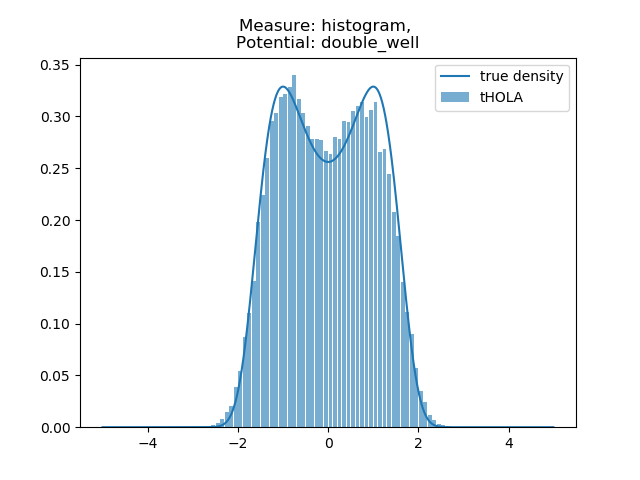
\includegraphics[width=\textwidth]{Figures/histo_example.png}
  \end{minipage} %
  \begin{minipage}[b]{0.3\textwidth}
  \centering
    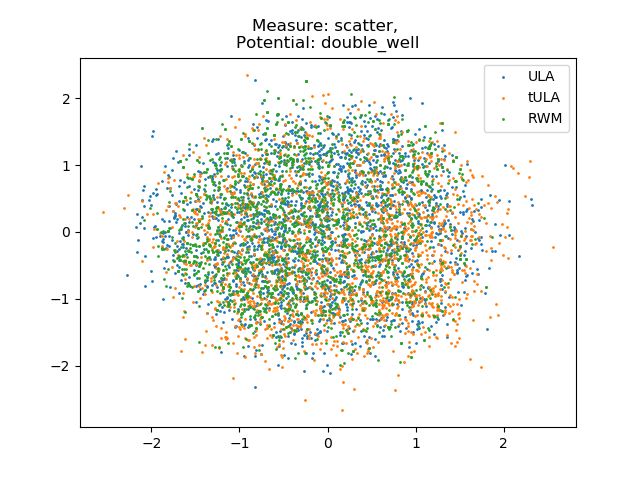
\includegraphics[width=\textwidth]{Figures/scatter_example.png}
  \end{minipage} %
  \begin{minipage}[b]{0.3\textwidth}
  \centering
    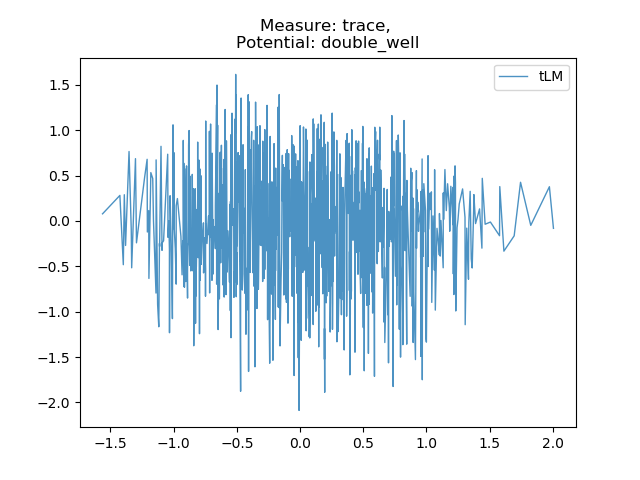
\includegraphics[width=\textwidth]{Figures/trace_example.png}
  \end{minipage}
   \caption{Example of a histogram plot, scatter plot and a trace plot.}
\end{figure}



\subsubsection{First/Second moments}
The first and second moments are implemented in the standard way. By default, the result is computed \textit{in the first coordinate only\footnote{With option to use $\frac 1 N\sum_{i=1}^N \norm{x_i}$ and $\frac 1 N\sum_{i=1}^N \norm{x_i^2}$ instead.}}.

$$ 
    \text{first moment} = \frac 1 N\sum_{i=1}^N x_i(1) \qquad \text{ and } \qquad \text{second moment} = \frac 1 N\sum_{i=1}^N x_i(1)^2
$$


\subsubsection{Total variation}
The total variation, being the first of implemented histogram measures, is calculated as

\[\text{total variation} = \norm{H_X - \frac 1 Z \sum_{c \in \#_X} \pi(c) \delta_c}_{\text{TV}} = \frac 1 2\sum_{c \in \#_X} \left|\frac{h(c)}{N} - \frac{\pi(c)}{Z}\right| .\]

\subsubsection{KL Divergence}
The next histogram-based measure is KL divergence.

\[\text{KL divergence} = D_{\text{KL}} \left( \frac 1 Z \sum_{c \in \#_X} \pi(c) \delta_c \,\bigg|\bigg| \, H_X) =  \sum_{c \in \#_X} \frac{\pi(c)}{Z} \log\left(\frac{\pi(c) N}{h(c) Z} \right)\right) .\]

\subsubsection{Sliced Wasserstein}

The Sliced Wasserstein distance, being defined via a multi-dimensional integral, cannot be computed exactly. Therefore, we resort to a simple Monte Carlo scheme where $L$ samples $\{\theta_i\}$ are drawn uniformly from the $(d-1)$-dimensional sphere $\mathbb S^{d-1}$.

$$ 
SW_p(P, Q) \approx \left( \frac 1 L \sum_{i=1}^L W_p^p\left(\mathcal{RI}_P(\cdot, \theta_i), \mathcal{RI}_Q(\cdot, \theta_i) \right) \right)^{\frac 1 p}
$$

The first, histogram based, implemented metric for Sliced Wasserstein distance further approximates the above Monte Carlo scheme for $SW_1$ as

\[\text{SW}_{histogram} = \begin{cases}
W_1 \left( H_X,\  \frac 1 Z \sum_{c \in \#_X} \pi(c) \delta_c \right) & \text{if dimension } = 1 \\
\sum_{i = 1}^L W_1 \left( \frac 1 N \sum_{c \in \#_X} h(c) \delta_{\left<c, \theta_i \right>},\  \frac 1 Z \sum_{c \in \#_X} \pi(c) \delta_{\left<c, \theta_i \right>}  \right) & \text{ otherwise, }
\end{cases}\]

where $\left< \cdot \right>$ is the dot product, $\theta_i = \frac{\theta'_i}{\norm{\theta'_i}}$ is a point on $(d-1)$-dimensional sphere with $
\theta'_i \sim \mathcal N(0, I_D)$ and $W_1$ is computed explicitly. \\\\

The second, \textbf{heuristic-based}, approximation of the Sliced Wasserstein distance is calculated as follows:

\[\text{SW}_{no\ histogram} = \begin{cases}
W_1 \left( \frac 1 N \sum_{x \in X} \delta_x,\  \frac 1 {Z'} \sum_{x \in X} \pi(x) \delta_x \right) & \text{if dimension } = 1 \\
\sum_{i = 1}^L W_1 \left(  \frac 1 N \sum_{x \in X} \delta_{\left<x, \theta_i \right>},\ \frac 1 {Z'} \frac 1 N \sum_{x \in X} \pi(x) \delta_{\left<x, \theta_i \right>}  \right) & \text{ otherwise. }
\end{cases}\]
where $Z' = \sum_{x \in X} \pi(x) $ is a normalizing constant. Intuitivelly, this measure of error describes whether the spatial distribution of samples is proportional to the true distribution, \textit{at the same points}.


\subsection{KDE-based metrics}

All three of the above histogram-based metrics are available in their KDE version as well. 

\[\text{total variation}^{\text{KDE}} = \norm{\text{KDE}_X - \frac 1 Z \sum_{c \in \#_X} \pi(c) \delta_c}_{\text{TV}} \]

\[\text{KL divergence}^{\text{KDE}} = D_{\text{KL}} \left(\text{KDE}_X \ \bigg|\bigg|\  \frac 1 Z \sum_{c \in \#_X} \pi(c) \delta_c\right) \]

\[\text{SW}_{histogram}^{\text{KDE}} = \begin{cases}
W_1 \left( \text{KDE}_X,\  \frac 1 Z \sum_{c \in \#_X} \pi(c) \delta_c \right) & \text{if dimension } = 1 \\
\sum_{i = 1}^L W_1 \left( \frac 1 {\hat Z} \sum_{c \in \#_X} \hat{\pi}_X(c) \delta_{\left<c, \theta_i \right>},\  \frac 1 Z \sum_{c \in \#_X} \pi(c) \delta_{\left<c, \theta_i \right>}  \right) & \text{ otherwise. }
\end{cases}\]